% gjilguid2e.tex
% V2.0 released 1998 December 18
% V2.1 released 2003 October 7 -- Gregor Hutton, updated the web address for the style files.

\documentclass[extra,mreferee]{gji}
\usepackage{timet}
\usepackage{gensymb}
\usepackage{graphicx}
\usepackage{float}
\usepackage{amsmath}
\usepackage[utf8]{inputenc}
%\usepackage{siunitx}

\title[Geophys.\ J.\ Int.: Magnetic radial inversion]
  {Magnetic data radial inversion for 3D source geometry estimation}
\author[L.B. Vital, V.C. Oliveira Jr., V.C.F. Barbosa]
  {L.B. Vital$^1$\thanks{Observatório Ncional, ON}\\
  $^1$ Observat{\'o}rio Nacional, Gal. Jos{\'e} Cristino, 77, São Crist{\'o}v{\~a}o,
  Rio de Janeiro, 20921-400, Brazil
  }
\date{Received 1998 December 18; in original form 1998 November 22}
\pagerange{\pageref{firstpage}--\pageref{lastpage}}
\volume{200}
\pubyear{1998}

%\def\LaTeX{L\kern-.36em\raise.3ex\hbox{{\small A}}\kern-.15em
%    T\kern-.1667em\lower.7ex\hbox{E}\kern-.125emX}
%\def\LATeX{L\kern-.36em\raise.3ex\hbox{{\Large A}}\kern-.15em
%    T\kern-.1667em\lower.7ex\hbox{E}\kern-.125emX}
% Authors with AMS fonts and mssymb.tex can comment out the following
% line to get the correct symbol for Geophysical Journal International.
\let\leqslant=\leq

\newtheorem{theorem}{Theorem}[section]

\begin{document}

\label{firstpage}

\maketitle


\begin{summary}
We present a method for inverting total-field anomaly data to estimate the geometry of a 3D complex geological source in subsurface. The method assumes magnetization vector and the depth to the top both known. We use an ensemble of vertically juxtaposed 3D right prisms to approximate the shape of the geological source. Each prism has a homogeneous known magnetization and an unknown polygon as its horizontal cross-sections. The vertices of the polygons approximately describe the edges of horizontal depth slices of the source. All prisms’ polygons have the same fixed number of vertices, which are equally spaced with central angles from $0^{\circ}$ to $360^{\circ}$ and horizontally described by polar coordinates associated to an arbitrary origin within each prism. The method estimates the radii of all vertices, the horizontal Cartesian coordinates of all arbitrary origins, and the depth extent of all prism defining the shape of the interpretation model. We impose zeroth- and first-order Tikhonov regularizations as constraints on the shape of the estimated model to stabilize the inverse problem. The method allows estimating both vertical and inclined sources by a suitable use of first-order Tikhonov regularization. This regularization can be applied on either all or few parameters excluding the depth extent of the prisms. The tests on synthetic total-field anomaly data show efficiency of the method on retrieving the shape of the source for either dipping
\end{summary}

\begin{keywords}
 Numerical solutions; Inverse theory; Magnetic anomalies.
\end{keywords}

\section{Introduction}


\section{Methodology}\label{sec:metodo}

\subsection{Forward problem}

Let $\mathbf{d}^o$ be the observed data (Fig. \ref{fig:obs}a), whose $i$th element $d^o_i$, $i = 1, \dots, N$, is the total-field anomaly measured at the point $(x_i, y_i, z_i)$ produced by a 3D source with known depth to the top. In a Cartesian coordinate system, wherein x points geographic north, y points east, and z points downward. We assume the total magnetization vector of the source is constant and known both its intensity and direction. We approximate the volume of the source by a set of $L$ vertically juxtaposed 3D prisms (Fig. \ref{fig:obs}b), like \cite{OliveiraJrVanderleiC.2011Sgeu} and \cite{OliveiraVanderleiC.20133rgg}. The depth to the top of the shallowest prism $z_0$ is defined by the interpreter based on the knowledge of the source. The magnetization vector of each prism $\mathbf{m}^k$, $k=1,\dots ,L$, is assumed constant and known. The horizontal cross-section of each prism is described by an arbitrary and unknown polygon with a fixed number $V$ of vertices equally spaced from $0^{\circ}$ to $360^{\circ}$, whose sides describe the edges of the horizontal depth slices of the source. The vertices of the polygon are described in polar coordinates referred to an arbitrary origin $O^k$ within the polygon. 

The radii of the vertices ($r^k_j$, $j=1,\dots , V$, $k=1,\dots ,L$), the horizontal coordinates ($x_0^k$ and $y_0^k$, $k=1,\dots ,L$) of the arbitrary origins $O^k$, $k=1,\dots ,L$, and the depth extent $dz$ of the L vertically stacked prisms in the ensemble are arranged in a $M$-dimensional vector $\mathbf{p}$, $M = L (V + 2) + 1$, given by
\begin{equation}
    \mathbf{p} =
    \left[ \begin{array}{@{}*{12}{c}@{}}
        r_1^1 & \dots & r_V^1 & x_0^1 & y_0^1 & \dots & r_1^L & \dots & r_V^L & x_0^L & y_0^L & dz\\
    \end{array} \right]^{\mathsf{T}},
\end{equation}
which will be estimated from the total-field anomaly data set.

\begin{figure}
    \centering
    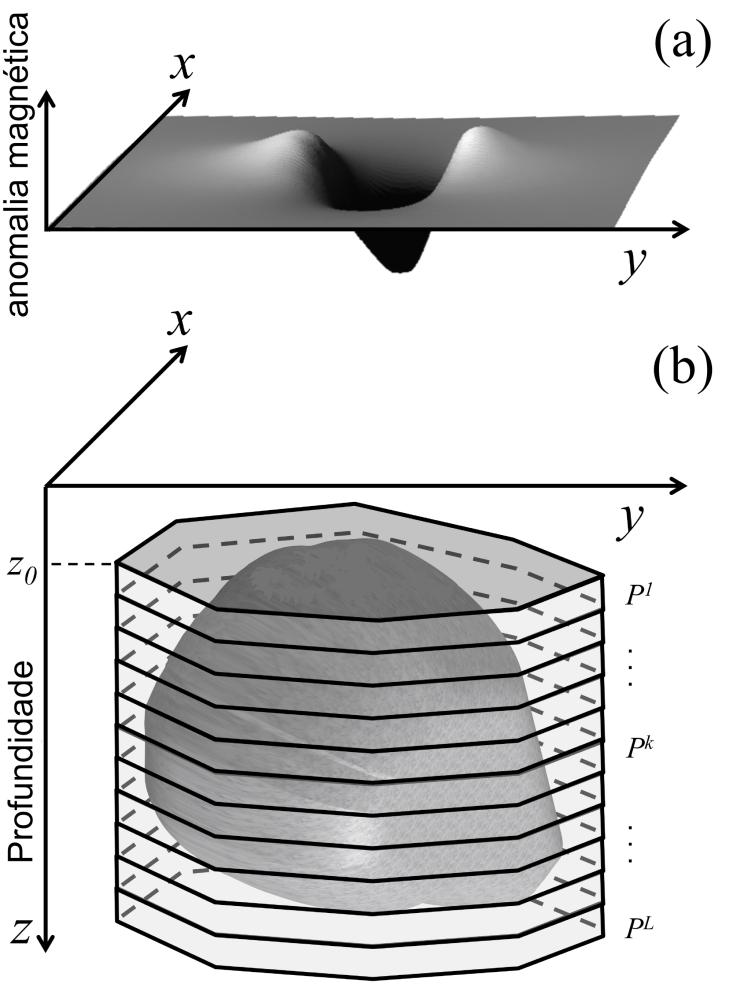
\includegraphics[scale=0.3]{figures/observed_data.png}
    \caption{Schematic representation of (a) total-filed anomaly (grey surface) produced by (b) a 3-D anomalous source (dark grey volume). The interpretation model in (b) consists of a set of L vertical, juxtaposed 3-D prisms $P^k$ , $k = 1,\dots, L$, (light grey prisms) in the vertical direction of a right-handed coordinate system.}
    \label{fig:obs}
\end{figure}

\begin{figure}
    \centering
    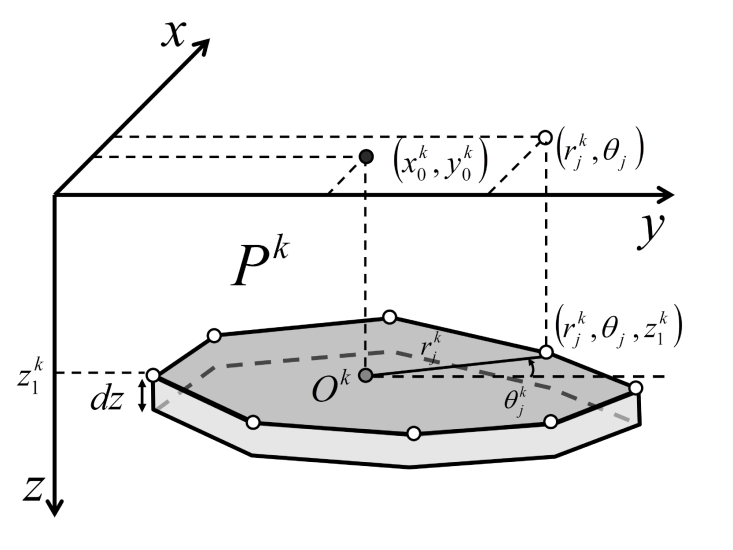
\includegraphics[scale=0.3]{figures/prism_parameters_mod.png}
    \caption{Polygonal cross-section of the $k$th vertical prism $P^k$ described by $V$ vertices (white dots) with polar coordinates ($r^k_j$ , $\theta ^k_j$), $j = 1, \dots, V$, $k = 1, \dots, L$ , referred to an arbitrary origin $O^k$ (grey dot) with horizontal Cartesian coordinates ($x_0^k$ , $y_0^k$), $k = 1, \dots, L$ , (black dot).}
    \label{fig:prism_parameters}
\end{figure}

The predicted total-field anomaly produced by the ensemble of L vertically stacked 3D prisms is the sum of the magnetic effect of each prism at the $i$th observation point ($x_i, y_i, z_i$)

\begin{equation}\label{eq:predicted}
d_i (\mathbf{p}) \equiv \sum\limits_{k=1}^L f_i^k(\mathbf{r}^k, x_0^k, y_0^k,\mbox{\boldmath$\theta$}, \mathbf{m}^k, z^k_1, dz), \quad i=1,\dots,N,
\end{equation}
where $\mathbf{r}^k$ and $\mbox{\boldmath$\theta$}$ are the $V$-dimensional vectors containing the polar coordinates of the vertices of the $k$th prism whose the $j$th components are $r^k_j$ and $\theta_j = (j-1)2\pi/V$, $j=1,\dots , V$, $k=1,\dots ,L$, respectively. Additionally, $\mathbf{m}^k$ is the magnetization vector of the $k$th prism $P^k$, whose depth to the top is given by $z_1^k = z_0 + (k-1)dz$. We calculated the the predicted total-field anomaly produced by the $k$th prism $P^k$, at the $i$th observation point ($x_i, y_i, z_i$), by using the Python package Fatiando a Terra \citep{uieda-proc-scipy-2013} which computes the non-linear function $f_i^k(\mathbf{r}^k, x_0^k, y_0^k,\mbox{\boldmath$\theta$}, \mathbf{m}^k, z^k_1, dz)$ based on the formulas proposed by \cite{PlouffD.1976Gamf}.

\subsection{Inverse problem}

The non-linear inversion of the total field anomaly consists in estimating the parameter vector $\mathbf{p}$ that minimizes the constrained objective function given by

\begin{equation}
\Gamma (\mathbf{p}) = \phi (\mathbf{p}) + \sum\limits^{7}_{\ell =1}\alpha_{\ell}\varphi_{\ell}(\mathbf{p}),
\label{eq:gamma}
\end{equation}
subject to
\begin{equation}\label{eq:desigualdade}
p_{n }^{min} < p_n < p_n^{max},\quad n =1, \dots, M,
\end{equation}
where $p_{n }^{min}$ and $p_n^{max}$ are the lower and upper limits for the $n$th element $p_n$ of the parameter vector $\mathbf{p}$, $\varphi (\mathbf{p})$ is the data-misfit function given by
\begin{equation}\label{eq:misfit}
\phi (\mathbf{p}) = \frac{1}{N}[\mathbf{d}^{o} - \mathbf{d}(\mathbf{p})]^2,
\end{equation}
where $\mathbf{d}(\mathbf{p})$ is a $N$-dimensional vector whose the $i$th element $d_i$ is the predicted total-field anomaly (equation~\ref{eq:predicted}) at the position $(x_i,y_i,z_i)$, $i = 1,\dots, N$.

The limits for the radii of all vertices of all prisms ($r^k_j$, $j=1,\dots , V$, $k=1,\dots ,L$), the horizontal Cartesian coordinates of all
arbitrary origins ($x_0^k$ , $y_0^k$ , $k = 1, \dots, L$), and the depth extent of all prisms $dz$ represented by $p_{n }^{min}$ and $p_n^{max}$ in the inequality constraints (equation \ref{eq:desigualdade}) are defined by the interpreter element by element based on both the horizontal extent of the magnetic anomaly and the knowledge about the source. 

To estimate a stable solution, we introduced a set of seven constraints on the geometry of the source. The $\ell$th constraint ($\ell = 1, \dots , 7$) is represented by the function $\phi_{\ell} (\mathbf{p})$ (equation \ref{eq:gamma}), where $\alpha_{\ell}$ is a positive scalar representing its weight. We use the Marquadt's method to minimize the objective function $\Gamma (\mathbf{p})$ (equation \ref{eq:gamma}) and introduce the inequality constraints (equation \ref{eq:desigualdade}) by using a strategy similar to that presented by \cite{BarbosaValeriaC.F.1999Gioa}. Our method imposes the constraints:
\begin{enumerate}
\item Smoothness constraint on the adjacent radii defining the horizontal section of each vertical prism. This constraint imposes that adjacent radii within each prism must be close to each other. It forces the estimated prism to be approximately cylindrical. %Accurately, it requires that the $j$th estimated radius $\hat{r}_j^k$ must be as close as possible to its consecutive radius $\hat{r}_{j+1}^k$ within the $k$th vertical prism. In other words, this constraint avoids an abrupt change between two consecutive radii. 
The matrix form of the this constraint is given by
\begin{equation}\label{eq:phi1m}
\varphi_{1}(\mathbf{p}) = \mathbf{p}^\mathsf{T}\mathbf{R}^\mathsf{T}_{1}\mathbf{R}_{1}\mathbf{p},
\end{equation}
where 
\begin{equation}
\mathbf{R}_{1} = 
\begin{bmatrix}
\mathbf{R}^{\sharp} & \mathbf{0}^{\sharp} & \mathbf{0}^{\sharp} & \cdots & \mathbf{0}^{\sharp} & \mathbf{0} \\
\mathbf{0}^{\sharp} & \textbf{R}^{\sharp} & \mathbf{0}^{\sharp} &  \cdots & \mathbf{0}^{\sharp} & \mathbf{0}\\
\mathbf{0}^{\sharp} & \mathbf{0}^{\sharp} & \ddots &  & \mathbf{0}^{\sharp} & \mathbf{0}\\
\vdots & \vdots &  & \ddots & \vdots & \vdots\\
\mathbf{0}^{\sharp} & \mathbf{0}^{\sharp} &  \cdots & \cdots & \mathbf{R}^{\sharp} & \mathbf{0}\\
\end{bmatrix}_{VL\times M},
\end{equation}
where $\mathbf{0}$ is a null column matrix with size $V+2$ and $\mathbf{0}^{\sharp}$ is a null matrix with the same shape of $\mathbf{R}^{\sharp}$ which is defined by 
\begin{equation}
\mathbf{R}^{\sharp} = 
\begin{bmatrix}
1 & -1 & 0 & 0 & \cdots & 0 & 0 & 0 & 0 \\
0 & 1 & -1 & 0 & \cdots & 0 & 0 & 0 & 0 \\
\vdots & \vdots & \vdots & \vdots & & \vdots & \vdots & \vdots & \vdots \\
0 & 0 & 0 & 0 & \cdots & 1 & -1 & 0 & 0 \\
-1 & 0 & 0 & 0 & \cdots & 0 & 1 & 0 & 0 \\
\end{bmatrix}_{V(L-1)\times (V+2)};
\end{equation}


\item Smoothness constraint on the adjacent radii of the vertically adjacent prisms. This constraint imposes that adjacent radii within vertically adjacent prisms must be close to each other. It forces the shape of all the estimated prisms to be similar. The matrix form of the this constraint is given by
\begin{equation}
\varphi_{2}(\mathbf{p}) = \mathbf{p}^\mathsf{T}\mathbf{R}^\mathsf{T}_{2}\mathbf{R}_{2}\mathbf{p} ,
\end{equation}
where
\begin{equation}
\mathbf{R}_{2} = 
\begin{bmatrix}
\mathbf{R}^{-}_{2} & \mathbf{R}^{+}_{2} & \mathbf{0}^{*} & \mathbf{0}^{*} & \cdots & \mathbf{0}^{*} & \mathbf{0}^{*} & \mathbf{0}\\
\mathbf{0}^{*} & \mathbf{R}^{-}_{2} & \mathbf{R}^{+}_{2} & \mathbf{0}^{*} & \cdots & \mathbf{0}^{*} & \mathbf{0}^{*} & \mathbf{0}\\
\mathbf{0}^{*} & \mathbf{0}^{*} & \mathbf{0}^{*} &  &  & \vdots & \vdots & \vdots\\
\vdots & \vdots & \vdots &  &  & \vdots & \vdots & \vdots\\
\mathbf{0}^{*} & \mathbf{0}^{*} & \mathbf{0}^{*} & \cdots & \cdots & \mathbf{R}^{-}_{2} & \mathbf{R}^{+}_{2} & \mathbf{0}\\
\end{bmatrix}_{V(L-1)\times M},
\end{equation}
where $\mathbf{0}^{*}$ is a null matrix with the same shape of $\mathbf{R}^{-}_2$ and $\mathbf{R}^{+}_2$ which are defined by 
\begin{equation}
\mathbf{R}^{-}_{2} = 
\begin{bmatrix}
-1 & 0 & 0 & \cdots & 0 & 0 \\
0 & -1 & 0 & \cdots & 0 & 0 \\
0 & 0 & \ddots &  & \vdots & \vdots \\
\vdots & \vdots  &  & \ddots & \vdots & \vdots\\
0 & 0 & \cdots & 0 & -1 & 0 \\
\end{bmatrix}_{V\times (V+2)}
\end{equation}
and
\begin{equation}
\mathbf{R}^{+}_{2} = 
\begin{bmatrix}
1 & 0 & 0 & \cdots & 0 & 0 \\
0 & 1 & 0 & \cdots & 0 & 0 \\
0 & 0 & \ddots &  & \vdots & \vdots \\
\vdots & \vdots  &  & \ddots & \vdots & \vdots\\
0 & 0 & \cdots & 0 & 1 & 0 \\
\end{bmatrix}_{V\times (V+2)};
\end{equation}

\item The source’s outcrop constraint. In the case of outcropping sources, this constraint imposes that the estimated horizontal cross-section of the shallowest prism must be close to the intersection of the geologic source with the known outcropping boundary. The matrix form of the this constraint is given by
\begin{equation}
\varphi_{3}(\mathbf{p}) = \left(\mathbf{A}\mathbf{p} - \mathbf{p}"\right)^\mathsf{T}\left(\mathbf{A}\mathbf{p} - \mathbf{p}"\right) ,
\end{equation}
where $\mathbf{p}"$ is a vector containing the parameters defining the polygon that represents the outcropping body given by
\begin{equation}
\mathbf{p}" = 
\begin{bmatrix}
r_{1}^{0} \\
r_{2}^{0} \\
\vdots \\
r_{M}^{0} \\
x_{0}^{0} \\
y_{0}^{0}
\end{bmatrix}_{(V+2)\times 1},
\end{equation}
and

\begin{equation}
\mathbf{A} = 
\begin{bmatrix}
\mathbf{I} & \hat{\mathbf{0}} \\
\end{bmatrix}_{(V+2)\times M},
\end{equation}
where $\mathbf{I}$ is an identity matrix with shape $V+2$ and $\hat{\mathbf{0}}$ is null matrix with shape $M -(V+2)$;

\item The source's horizontal location constraint. In the case of outcropping sources, this constraint imposes that the estimated horizontal Cartesian coordinates of the arbitrary origin within the shallowest prism must be as close as possible to the known horizontal Cartesian coordinates of a point on the outcropping body. The matrix form of the this constraint is given by
\begin{equation}
\varphi_{4}(\mathbf{p}) = \left(\mathbf{B}\mathbf{p} - \mathbf{p}'\right)^\mathsf{T}\left(\mathbf{B}\mathbf{p} - \mathbf{p}'\right) ,
\end{equation}
where
\begin{equation}
\mathbf{B} = 
\begin{bmatrix}
\mathbf{B}^{\sharp} & \hat{\mathbf{0}} \\
\end{bmatrix}_{2\times M} ,
\end{equation}

\begin{equation}
\textbf{B}^{\sharp} = 
\begin{bmatrix}
0 & \cdots & 0 & 1 & 0 \\
0 & \cdots & 0 & 0 & 1
\end{bmatrix}_{2\times (V+2)},
\end{equation}
and $\textbf{p}'$ is a vector containing the Cartesian coordinates of the horizontal location of the source given by

\begin{equation}
\textbf{p}' = 
\begin{bmatrix}
x^0_0 \\
y^0_0
\end{bmatrix}_{2\times 1} ;
\end{equation}

\item Smoothness constraint on the horizontal position of the arbitrary origins of the vertically adjacent prisms. This constraint imposes that the estimated horizontal Cartesian coordinates of vertically adjacent prisms must be close to each other. It forces the estimated prisms to be approximately vertically aligned. The matrix form of the this constraint is given by
\begin{equation}
\varphi_{5}(\textbf{p}) = \textbf{p}^\mathsf{T}\textbf{R}^\mathsf{T}_{5}\textbf{R}_{5}\textbf{p} ,
\end{equation}
where
\begin{equation}
\mathbf{R}_{5} = 
\begin{bmatrix}
\mathbf{R}^{-}_{5} & \mathbf{R}^{+}_{5} & \mathbf{0}^{\pm} & \mathbf{0}^{\pm} & \cdots & \mathbf{0}^{\pm} & \mathbf{0}^{\pm} & \mathbf{0}\\
\mathbf{0}^{\pm} & \mathbf{R}^{-}_{5} & \mathbf{R}^{+}_{5} & \mathbf{0}^{\pm} & \cdots & \mathbf{0}^{\pm} & \mathbf{0}^{\pm} & \mathbf{0}\\
\mathbf{0}^{\pm} & \mathbf{0}^{\pm} & \mathbf{0}^{\pm} &  &  & \vdots & \vdots & \vdots\\
\vdots & \vdots & \vdots &  &  & \vdots & \vdots & \vdots\\
\mathbf{0}^{\pm} & \mathbf{0}^{\pm} & \mathbf{0}^{\pm} & \cdots & \cdots & \mathbf{R}^{-}_{5} & \mathbf{R}^{+}_{5} & \mathbf{0}\\
\end{bmatrix}_{2(L-1)\times M},
\end{equation}
where $\mathbf{0}^{\pm}$ is a null matrix with the same shape of $\mathbf{R}^{-}_{5}$ and $\mathbf{R}^{+}_{5}$ which are given by
\begin{equation}
\textbf{R}^{-}_{5} = 
\begin{bmatrix}
0 & 0 & \cdots & 0 & -1 & 0 \\
0 & 0 & \cdots & 0 & 0 & -1 \\
\end{bmatrix}_{2\times (V+2)},
\end{equation}

\begin{equation}
\textbf{R}^{+}_{5} = 
\begin{bmatrix}
0 & 0 & \cdots & 0 & 1 & 0 \\
0 & 0 & \cdots & 0 & 0 & 1 \\
\end{bmatrix}_{2\times (V+2)};
\end{equation}

\item Minimum Euclidean norm constraint on the adjacent radii within each vertical prism. This constraint imposes that all estimated radii within each prism must be close to null values. The matrix form of the this constraint is given by
\begin{equation}
\varphi_{6}(\textbf{p}) = \textbf{p}^\mathsf{T}\textbf{C}^\mathsf{T}\textbf{C}\textbf{p},
\end{equation}
where
\begin{equation}
\textbf{C} = 
\begin{bmatrix}
\textbf{C}^{\sharp} & \mathbf{0} & \mathbf{0} & \cdots & \mathbf{0} & \mathbf{0}\\
\mathbf{0} & \textbf{C}^{\sharp} &  \mathbf{0} & \cdots & \mathbf{0} & \mathbf{0}\\
\mathbf{0} & \mathbf{0} & \ddots & & \vdots & \vdots\\
\vdots & \vdots & & \ddots & \vdots & \vdots\\
\mathbf{0} & \mathbf{0} &  \cdots & \cdots & \textbf{C}^{\sharp} & \mathbf{0}\\
\mathbf{0} & \mathbf{0} &  \cdots &  \cdots & \mathbf{0} & 0\\
\end{bmatrix}_{M\times M} ,
\end{equation}

\begin{equation}
\textbf{C}^{\sharp} = 
\begin{bmatrix}
1 & & & & \\
& \ddots &  & &  \\
&  & 1 & & \\
&  & & 0 &  \\
&  & & & 0 \\
\end{bmatrix}_{(V+2)\times (V+2)};
\end{equation}

\item Minimum Euclidean norm constraint on the depth extent of all prisms. This constraint imposes that the estimated depth extent of the prisms must be close to a null value. The matrix form of the this constraint is given by
\begin{equation}\label{eq:phi7}
\varphi_7 = \mathbf{p}^\mathsf{T}\mathbf{D}^\mathsf{T}\mathbf{D}\mathbf{p},
\end{equation}
where
\begin{equation}
\mathbf{D} =
\begin{bmatrix}
 0 & \cdots  & 0 \\
 \vdots & \ddots & \vdots\\
 0  & \cdots  & 1\\
\end{bmatrix}_{M\times M}.
\end{equation}

\end{enumerate}

Most of these constraints are defined by using the Tikhonov regularizing functions of order zero and one \citep{Aster2005}, by following the same approach presented by \cite{OliveiraJrVanderleiC.2011Sgeu}. Here, we present the constraint on the depth extent of all prisms.

\section{Synthetic tests}

To examine the performance of our inversion method, we present two applications with total-field anomaly data simulating two different isolated geological sources. The first source is a funnel-shaped model with a simple geometry, which satisfies all of the constraints described in Section \ref{sec:metodo}. The aim is to test the regularization in an ideal case with simple geometry. The second source has a complex geometry, which does not satisfy any constraint. The purpose, here, is to show that the constraints can stabilize the inverse problem in a more realistic case retrieving the geometry of the source with known magnetization using the polygonal prisms.

In both applications, the synthetic total-field anomaly was computed in an irregular grid on plane $z=-100$ m and contaminated with pseudorandom Gaussian noise sequences with mean zero and different standard deviation. In both cases, we considered the main magnetic field with inclination and declination of $50^\circ$ and $-15^\circ$, respectively. However, the simple model has only induced magnetization while the second model has a remnant magnetization specified below.

Although the simulated sources have a different depth to the top, we have considered both known. We also assumed the same magnetization for all prisms of the magnetic sources. On the other hand, the depth extent of the sources was not set in the initial guesses because it is a parameter for the inverse problem. Moreover, we have investigated the influence of the parameters from the initial guess on the solution by varying them and evaluating the effect on the misfit function.

\subsection{Simple model test}

The first synthetic source has $L=8$ prisms, each one with $M = 20$ vertices, and a purely induced magnetization with an intensity of $5$ A/m. Its depth to the top $z_0$ is at $50$ m and the bottom at $1250$ m. The radii of the vertices are equal within the same prism and decrease along with the depth with a step of $60$ m starting with $r_j^k=640$ m, $j=1,\dots, M$ (Figure \ref{fig:kimb}a). The horizontal coordinates $x_0$ and $y_0$ of the origins of the polygons $O^k$ are equal to $(0,0)$ for all prisms. We calculated the synthetic data produced by this source on an area of $16$ km$^2$, simulating an airborne survey composed of $16$ flight lines that are equally spaced from $200$ m to $1200$ m along the horizontal coordinate $y$, at a constant vertical coordinate $z=-100$ m (Figure \ref{fig:kimb}b).

For the inversion, we used an interpretation model formed by $L=6$ prisms, each one with $M=15$ vertices. The prisms forming the initial approximation have the same radii for all vertices ($500$ m) and depth extent ($220$ m), so the maximum depth is equal to $1320$ m. We have used all constraints described in Section 2 except the third and fourth constraints. We weighted the constraints with $\alpha_1 = 0.0006$, $\alpha_2 = 0.0006$, $\alpha_5 = 0.009$, $\alpha_6 = 0.00001$, and $\alpha_7 = 0.0001$. Both Cartesian coordinates $x_0^k$ and $y_0^k$ of the origins of all prisms $O^k$, $k=1,\dots,L$, are located at the point $(0,0)$. Fig. \ref{fig:kimb}c shows the result of the inversion of the noise-corrupted total-field anomaly in Fig. \ref{fig:kimb}b. The red prisms are very close to the edges of the true body (blue lines) even using fewer prisms than the true body has. Moreover, the estimated depth extent of each prism is $dz = 200.65$ m, which gives us a very accurate total depth extent of $1203.88$ m. Figure \ref{fig:kimb}d shows that the residuals have a mean mean very close to zero ($\mu=0.09$ nT) and a coherent standard deviation ($\sigma=5.23$ nT).

\begin{figure}
    \centering
    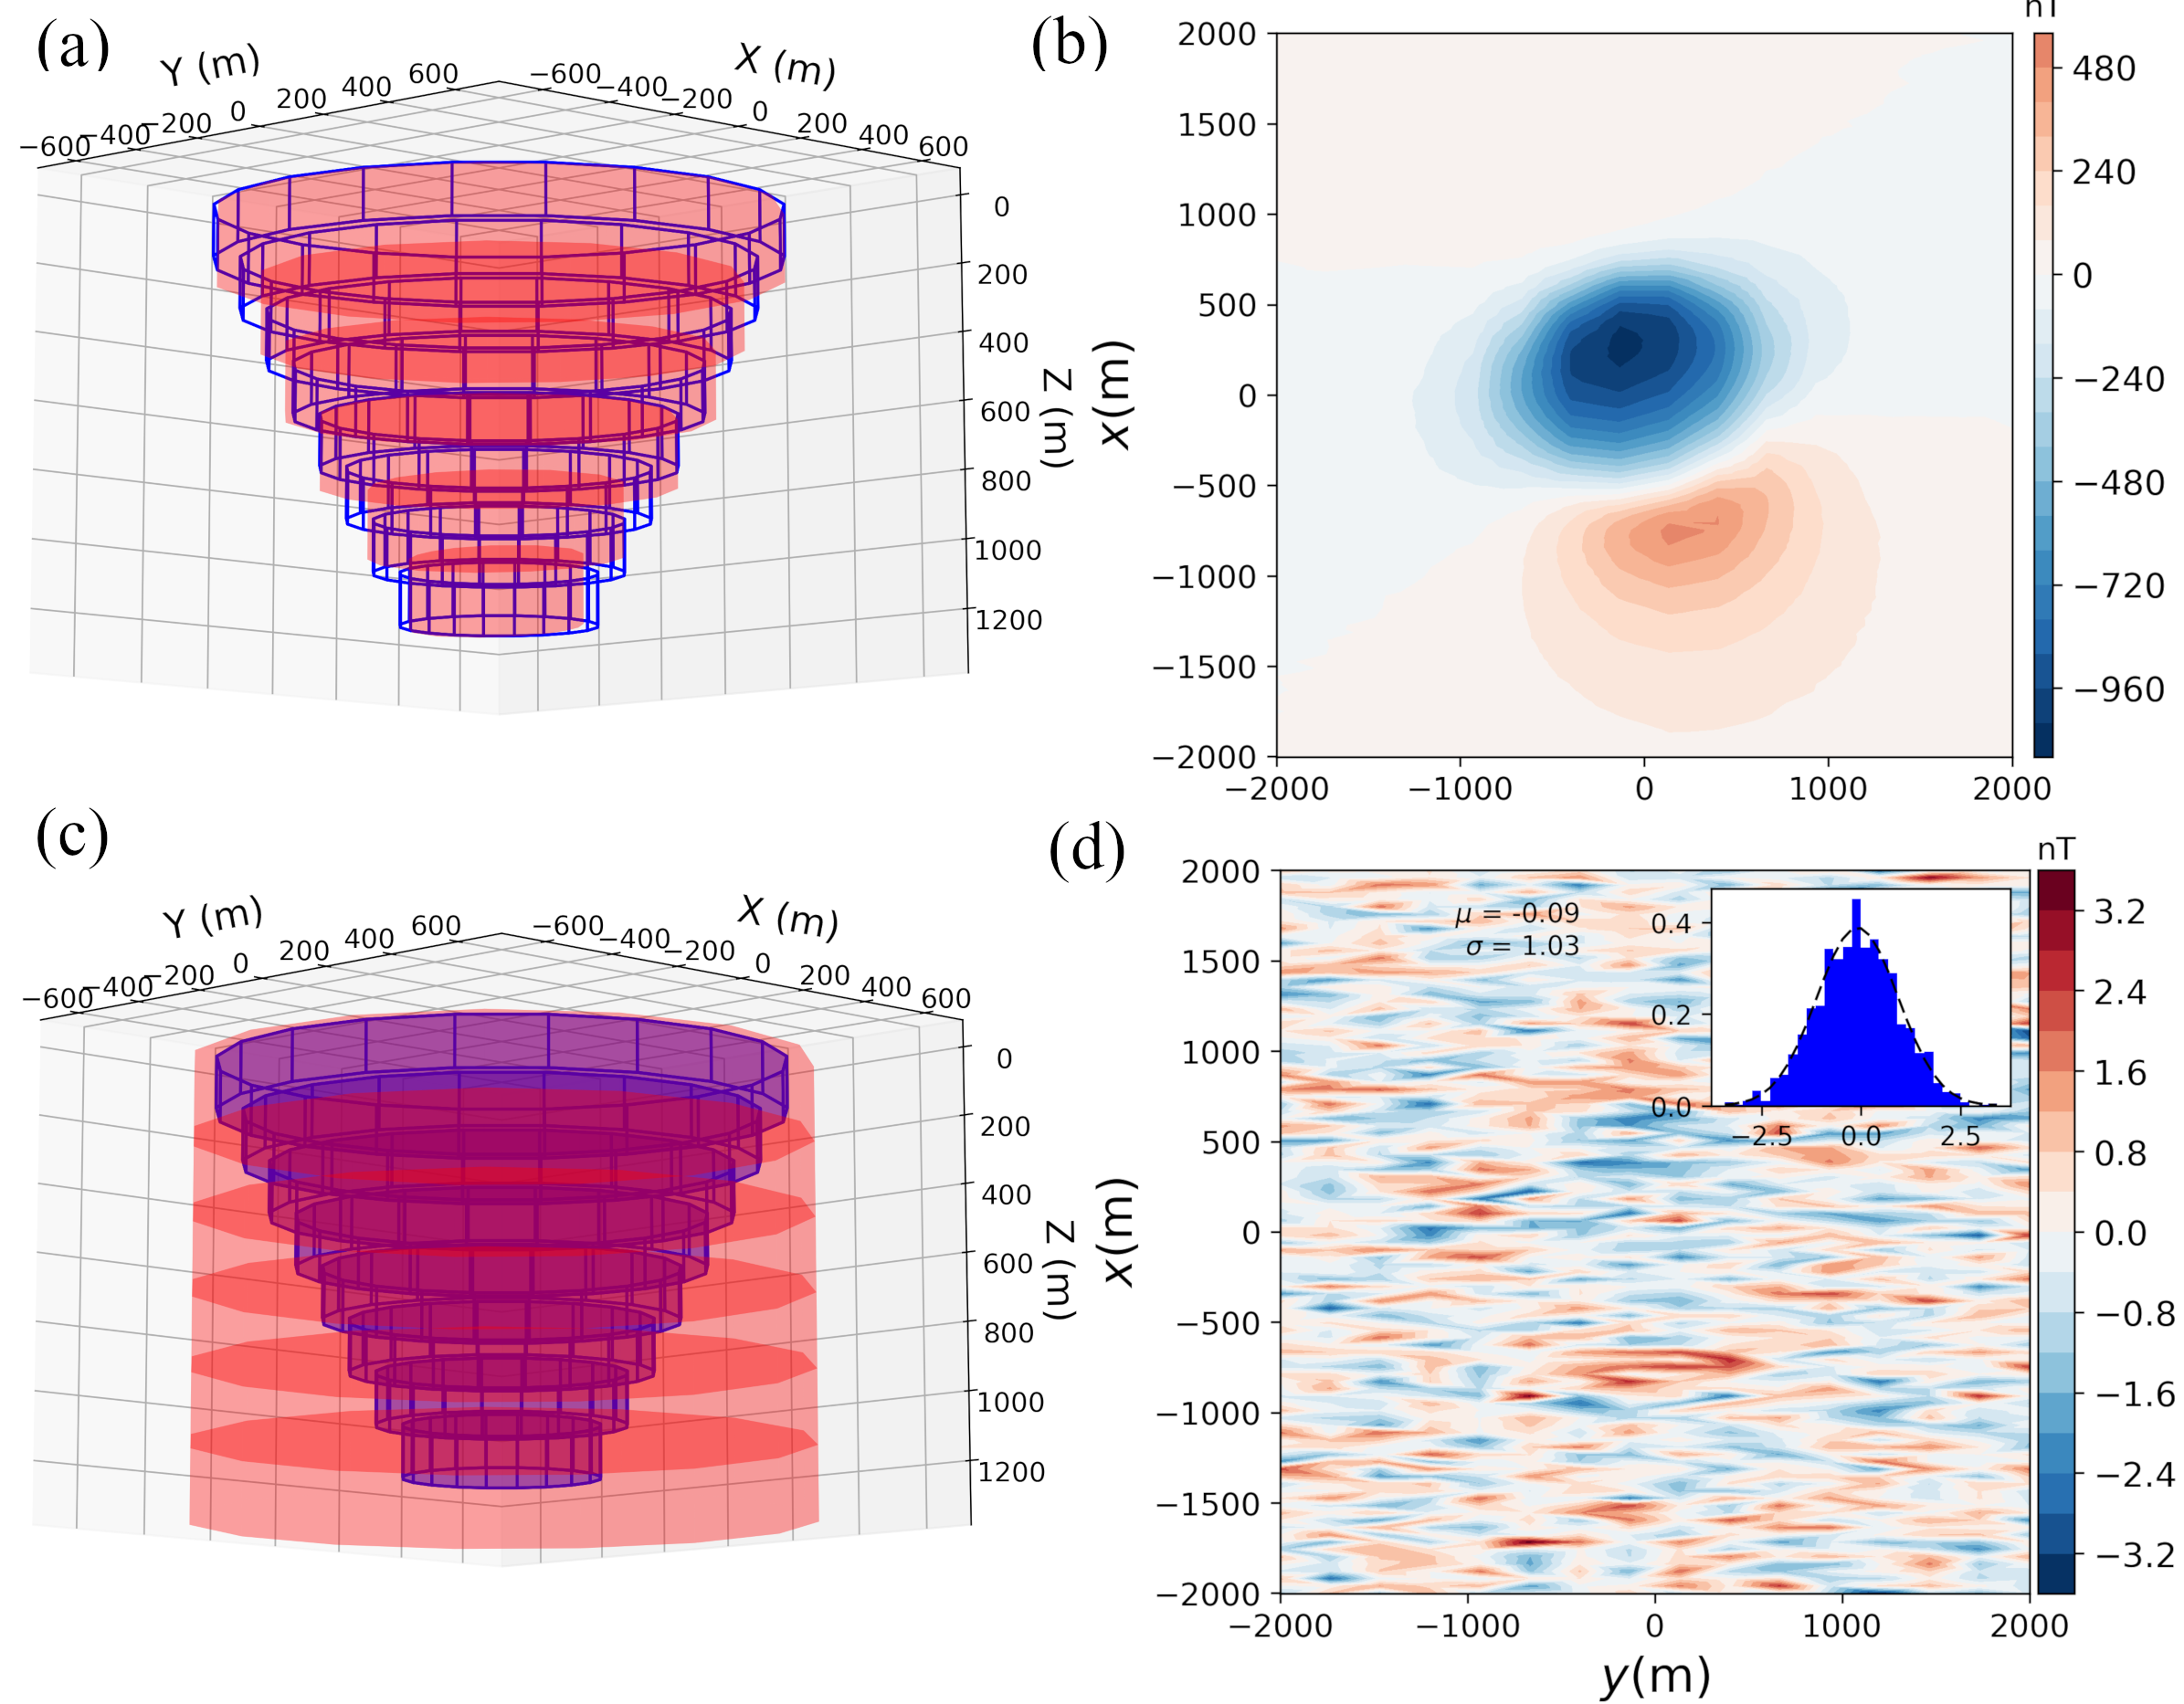
\includegraphics[scale=.75]{figures/kimberlite_4figures.png}
    \caption{(a) Perspective view of the simple model with the depth to the top $z_0 = 50$ m and the depth extent $1200$ m. (b) Synthetic noise-corrupted total-field anomaly produced by the simple model blue prisms in (a). The data was contaminated by a pseudorandom Gaussian noise with mean zero and standard deviation $1$ nT. (c) Perspective view of the true (blue lines) and estimated body (red prisms) obtained by inverting the noise-corrupted total-field anomaly in (b). (d) Residuals defined as the difference between the noisy and the predicted (not shown) total-field anomalies; the latter was produced by the estimated body (red prisms in b). The inset in d shows the histogram and the Gaussian curve for the residuals with mean $\mu=0.1$ nT and standard deviation $\sigma=5.23$ nT.
}
    \label{fig:kimb}
\end{figure}

\subsection{Complex model test}

The second synthetic source has $L=10$ prisms, each one with $M=30$ vertices, and a total magnetization with intensity $\|\mathbf{m}\| =10$ A/m. The complex model has both induced and remnant magnetization with inclination $65$º, and declination $-40.5$º. Its depth to the top $z_0$ is $200$ m and its bottom is at $4200$ m. The radii of the vertices ($r_j^k$, $j=1,\dots,M$, $k=1,\dots,L$) forming this synthetic body vary from $240$ to $1540$ m and the horizontal coordinates $x_0$ and $y_0$ of the origins of the polygons $O^k$ vary from $-250$ m and $250$ m to $750$ m and $-750$ m, respectively (Figure \ref{fig:complex_model}a) by an equal step for both of $100$ m. We calculated the synthetic data produced by this body, simulating an airborne survey covering an area of $100$ km$^2$ composed of 21 flight lines that are equally spaced from $-5000$ m to $5000$ m, along with the horizontal coordinate $y$, and with a height of $-100$ m (Figure \ref{fig:complex_model}b). The initial guess is a cylinder formed by $L=8$ prisms, each one with $M=15$ vertices centered at $(x_0^k, y_0^k) = (0,0)$. All prisms that form the initial approximation have the same radii ($500$ m) and depth extent ($600$ m) reaching $4800$ m of maximum depth(Figure \ref{fig:complex_model}a).

\begin{figure}
    \centering
    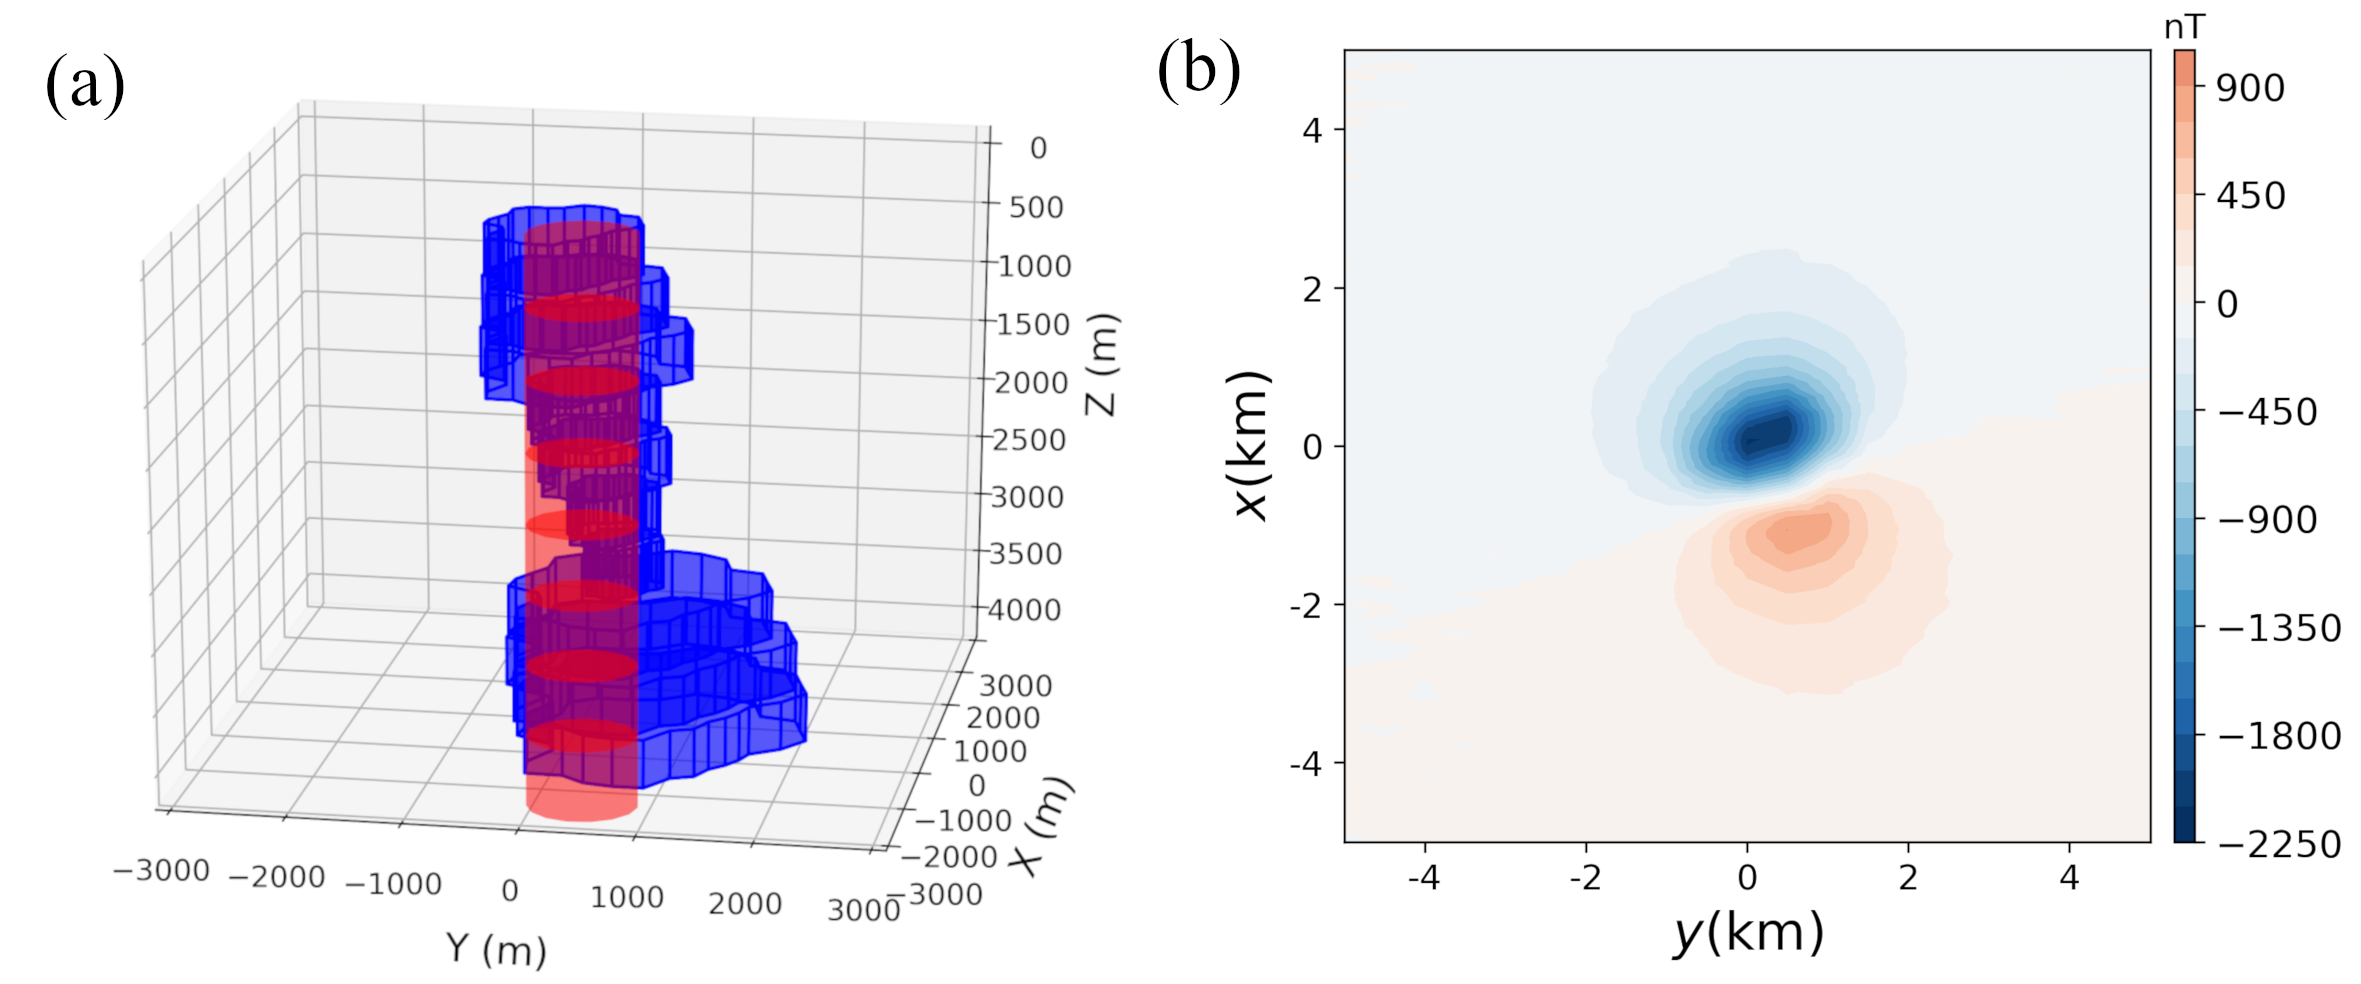
\includegraphics[scale=.75]{figures/complex_3d_ini_data.png}
    \caption{(a) Perspective view of the complex model (blue prisms) with the depth to the top $z_0 = 200$ m and the depth extent $4000$ m and the initial guess (red prisms) for the inversion which is a cylinder with radius $500$ m and depth extent $4800$ m. (b) Synthetic noise-corrupted total-field anomaly produced by the complex model blue prisms in (a). The data was contaminated by a pseudorandom Gaussian noise with mean zero and standard deviation $5$ nT.
}
    \label{fig:complex_model}
\end{figure}

We set the weights for the constraints $\alpha_1 = 0.0005$, $\alpha_2 = 0.003$, $\alpha_5 = 0.05$, $\alpha_6 = 0.00001$, and $\alpha_7 = 0.04$. Again, the third and fourth constraints were not used. Fig. \ref{fig:complex_result}a shows the result of the inversion of the noise-corrupted total-field anomaly in Fig. \ref{fig:complex_model}. Due to the lower number of prisms in the interpretation model, the estimated body does not retrieve perfectly the simulated body. However, the volume of the complex model is $8.40$ km$^3$, while the volume of the estimated source is $8.29$ km$^3$. Moreover, the estimated depth extent is $3875.4$ m, which is close to $4000$ m. The residuals have a mean and a standard deviation very close to the values of the noise also the histogram is coherent with a Gaussian distribution (Figure \ref{fig:complex_result})d.

\begin{figure}
    \centering
    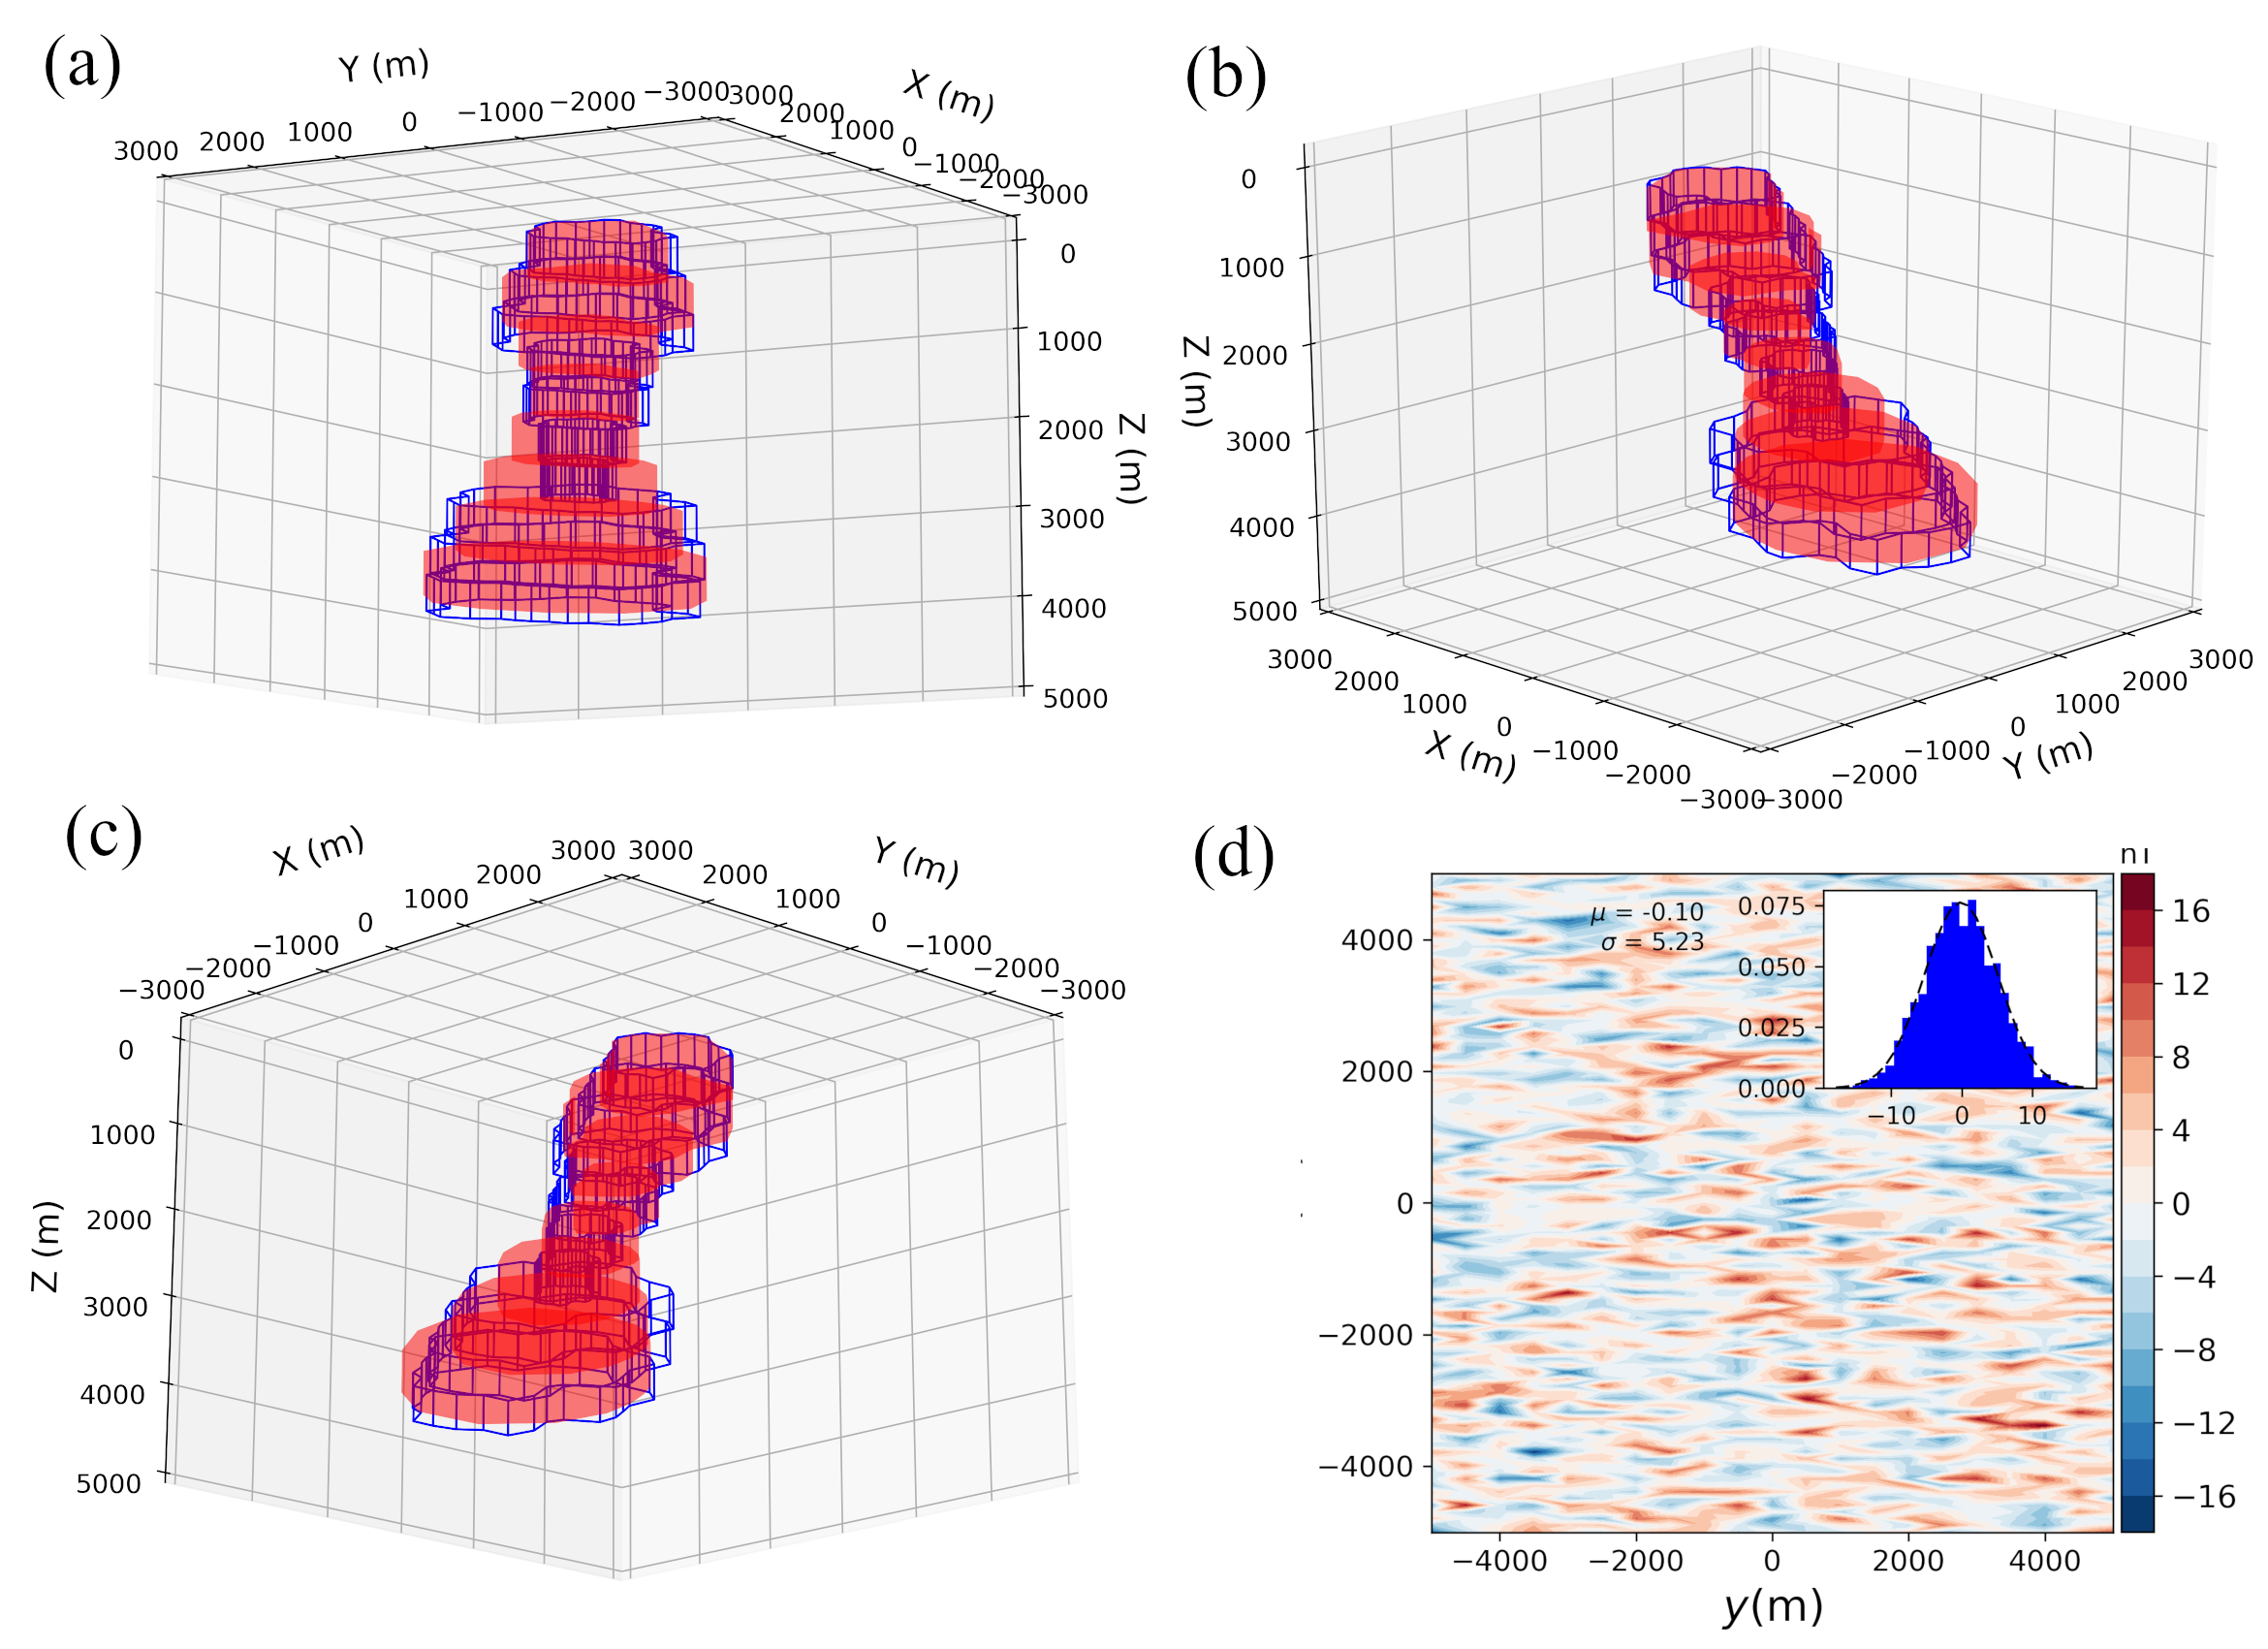
\includegraphics[scale=.75]{figures/complex_estimates_residual.png}
    \caption{Perspective views of the complex model (blue lines) and the estimate (red prisms) in (a), (b) and (c). (d) Residuals defined as the difference between the noisy and the predicted (not shown) total-field anomalies and the histogram of the residuals (inset in d) with mean $\mu=0.1$ nT and standard deviation $\sigma=5.23$ nT. The dashed line on the inset is the Gaussian curve for the residuals.
}
    \label{fig:complex_result}
\end{figure}


%In both tests, from the initial guesses (red prisms in Figures 4a e 5a), the method provided estimates that fit the data and retrieve the geometry of the simulated bodies (red prisms in Figures 4b and 5b). Overall, the method can closely estimate the geometries of the simulated bodies and their bottom depths. The acceptable data fittings yielded by the estimated bodies are confirmed by the small residuals shown in Figures 4c and 5c. In both tests, the residuals are smaller than  $\pm 0.34$ nT and $\pm 18$ nT which correspond to less than $1\%$ of the total amplitude of their data sets.


\section{Application to real data}

There is a region in the central part of Brazil where are occurrences of Cretaceous alkaline rocks along a lineament NW-SE. Authors have been studying this region since the 60s classifying it with different nomenclatures throughout the years. Recently, \cite{Junqueira-BrodTerezaCristina2002Apad} have proposed the nomenclature Goiás alkaline province (GAP) for the alkaline rocks close to Rio Verde and Iporá cities (in Goiás state). Mafic to ultramafic alkaline rocks form GAP complex surrounded by a Precrambian basement and Phanerozoic sedimentary rocks from Paraná basin. An aeromagnetic survey was flown in 2004 with an almost constant height of $100$ m from the terrain covering the region.  The N-S lines are spaced from 500 m and the tie E-W tie-lines are spaced from $5000$ m. The flight height was approximately constant at $100$ m above the terrain, and the interval between the measurements was $0.1$ s, this interval resulted in one measurement at each approximately $8$ m. However, we decimated the data by removing measurements that the interval between them is 88 m (Figure \ref{fig:real_data}). The diurnal variation correction and the Earth's main field subtraction were made on the data. The Earth's main field was subtracted using the International Geomagnetic Reference Field (IGRF) evaluated at the 2004.62 epoch, with declination $-18.5$º and inclination $-19.5$º.

\cite{OliveiraV2015Eott} estimated the source's total magnetization direction in the alkaline complex of Diorama under the premise of approximated spherical sources. They validated the estimated magnetization direction (inclination $-71.4$º and declination $-23.4$º) by computing the reduction to the pole of magnetic anomalies over the alkaline complexes of Diorama and Montes Claros de Goiás. To attenuate the non-dipolar effects present in the data, we applied the equivalent layer \citep{DampneyC.N.G.1969Test,EmiliaDavidA.1973Esua} to continue the anomaly upward to a constant normal height of 1100m. We applied our method on the Diorama upward continued total-field anomaly (not shown) by using an initial guess (blue prisms in Figure \ref{fig:real_result}) with $L=10$ prisms, each one with $M=30$ vertices, depth to the top $z_0=50$ m, $dz = 800$ m, and all radii are equal to $100$ m, total magnetization intensity $15$ A/m and direction equal to that estimated by \cite{OliveiraV2015Eott}. The estimated source (Figure \ref{fig:real_result}) reaches a maximum depth of about 6 km and has a very complex geometry. Although the data fitting produced by the estimated source may seem unacceptable because the large residuals (Figure \ref{fig:real_result}d) which range from $-64$ to $64$ nT, we stress that the misfit value is about to $9\%$.

\begin{figure}
    \centering
    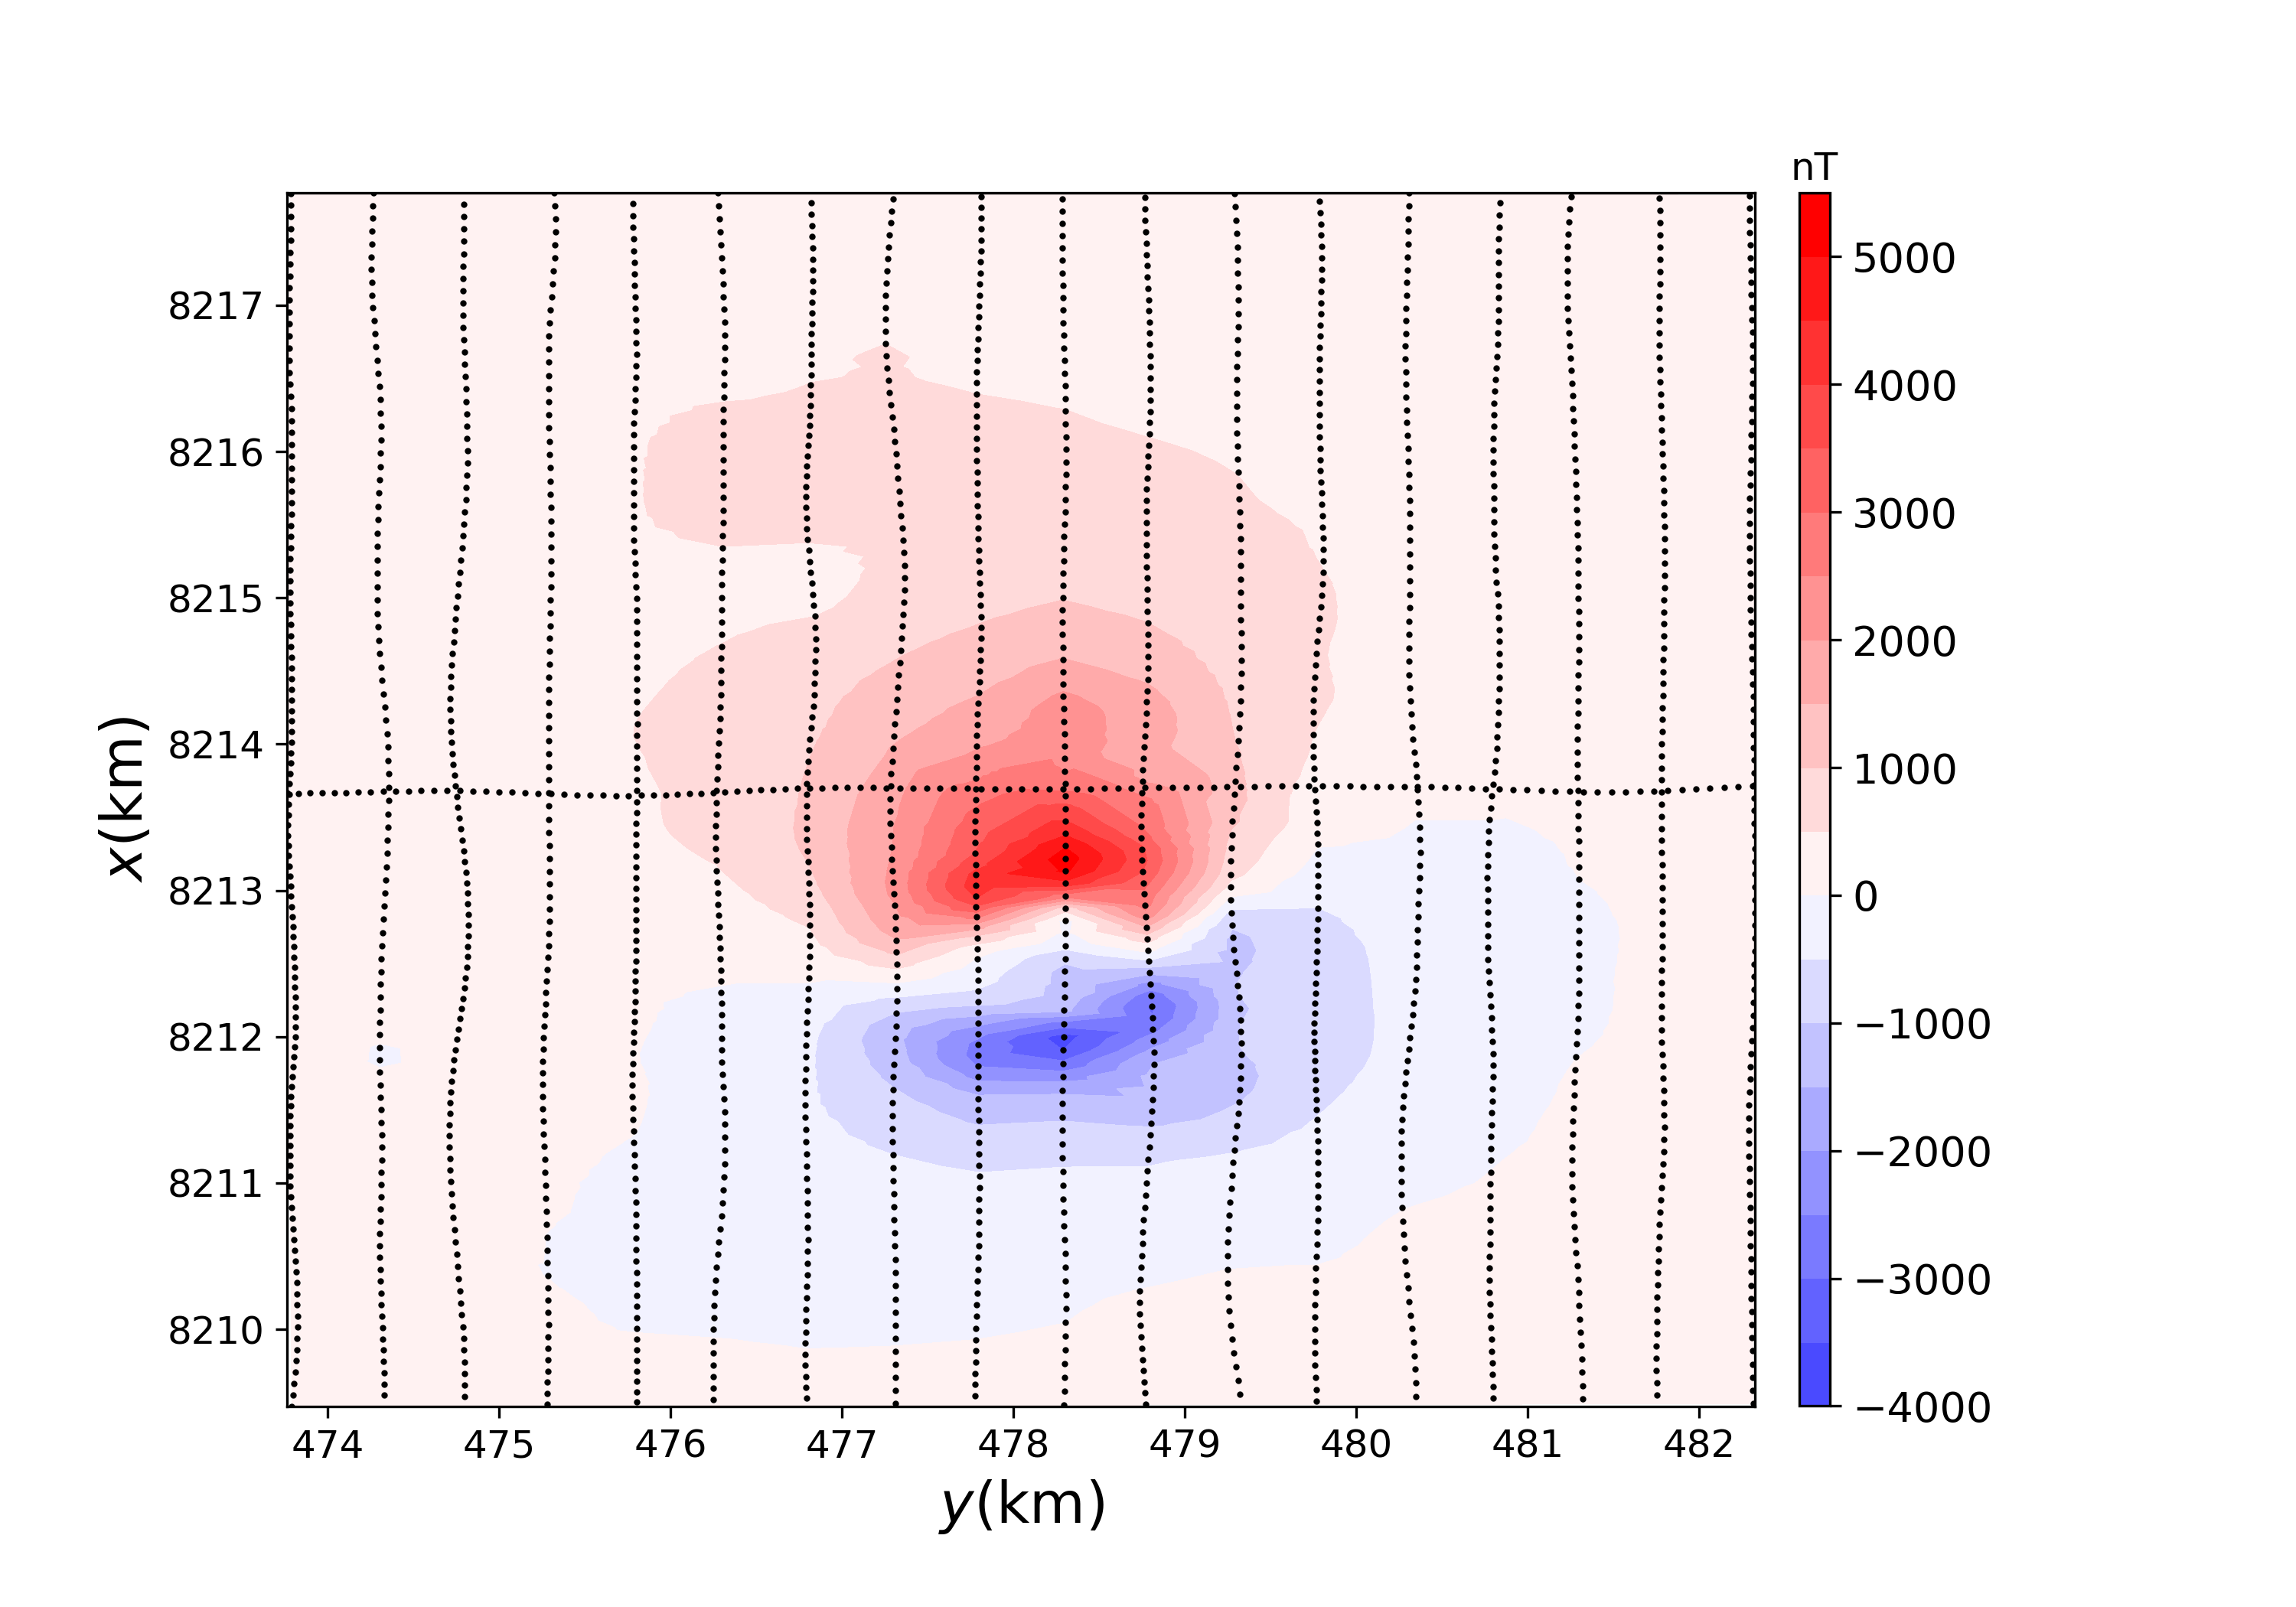
\includegraphics[scale=.5]{figures/diorama_real_data.png}
    \caption{Total-field anomaly of Diorama in GAP. The black dots are the observation points used in this work.
}
    \label{fig:real_data}
\end{figure}

\begin{figure}
    \centering
    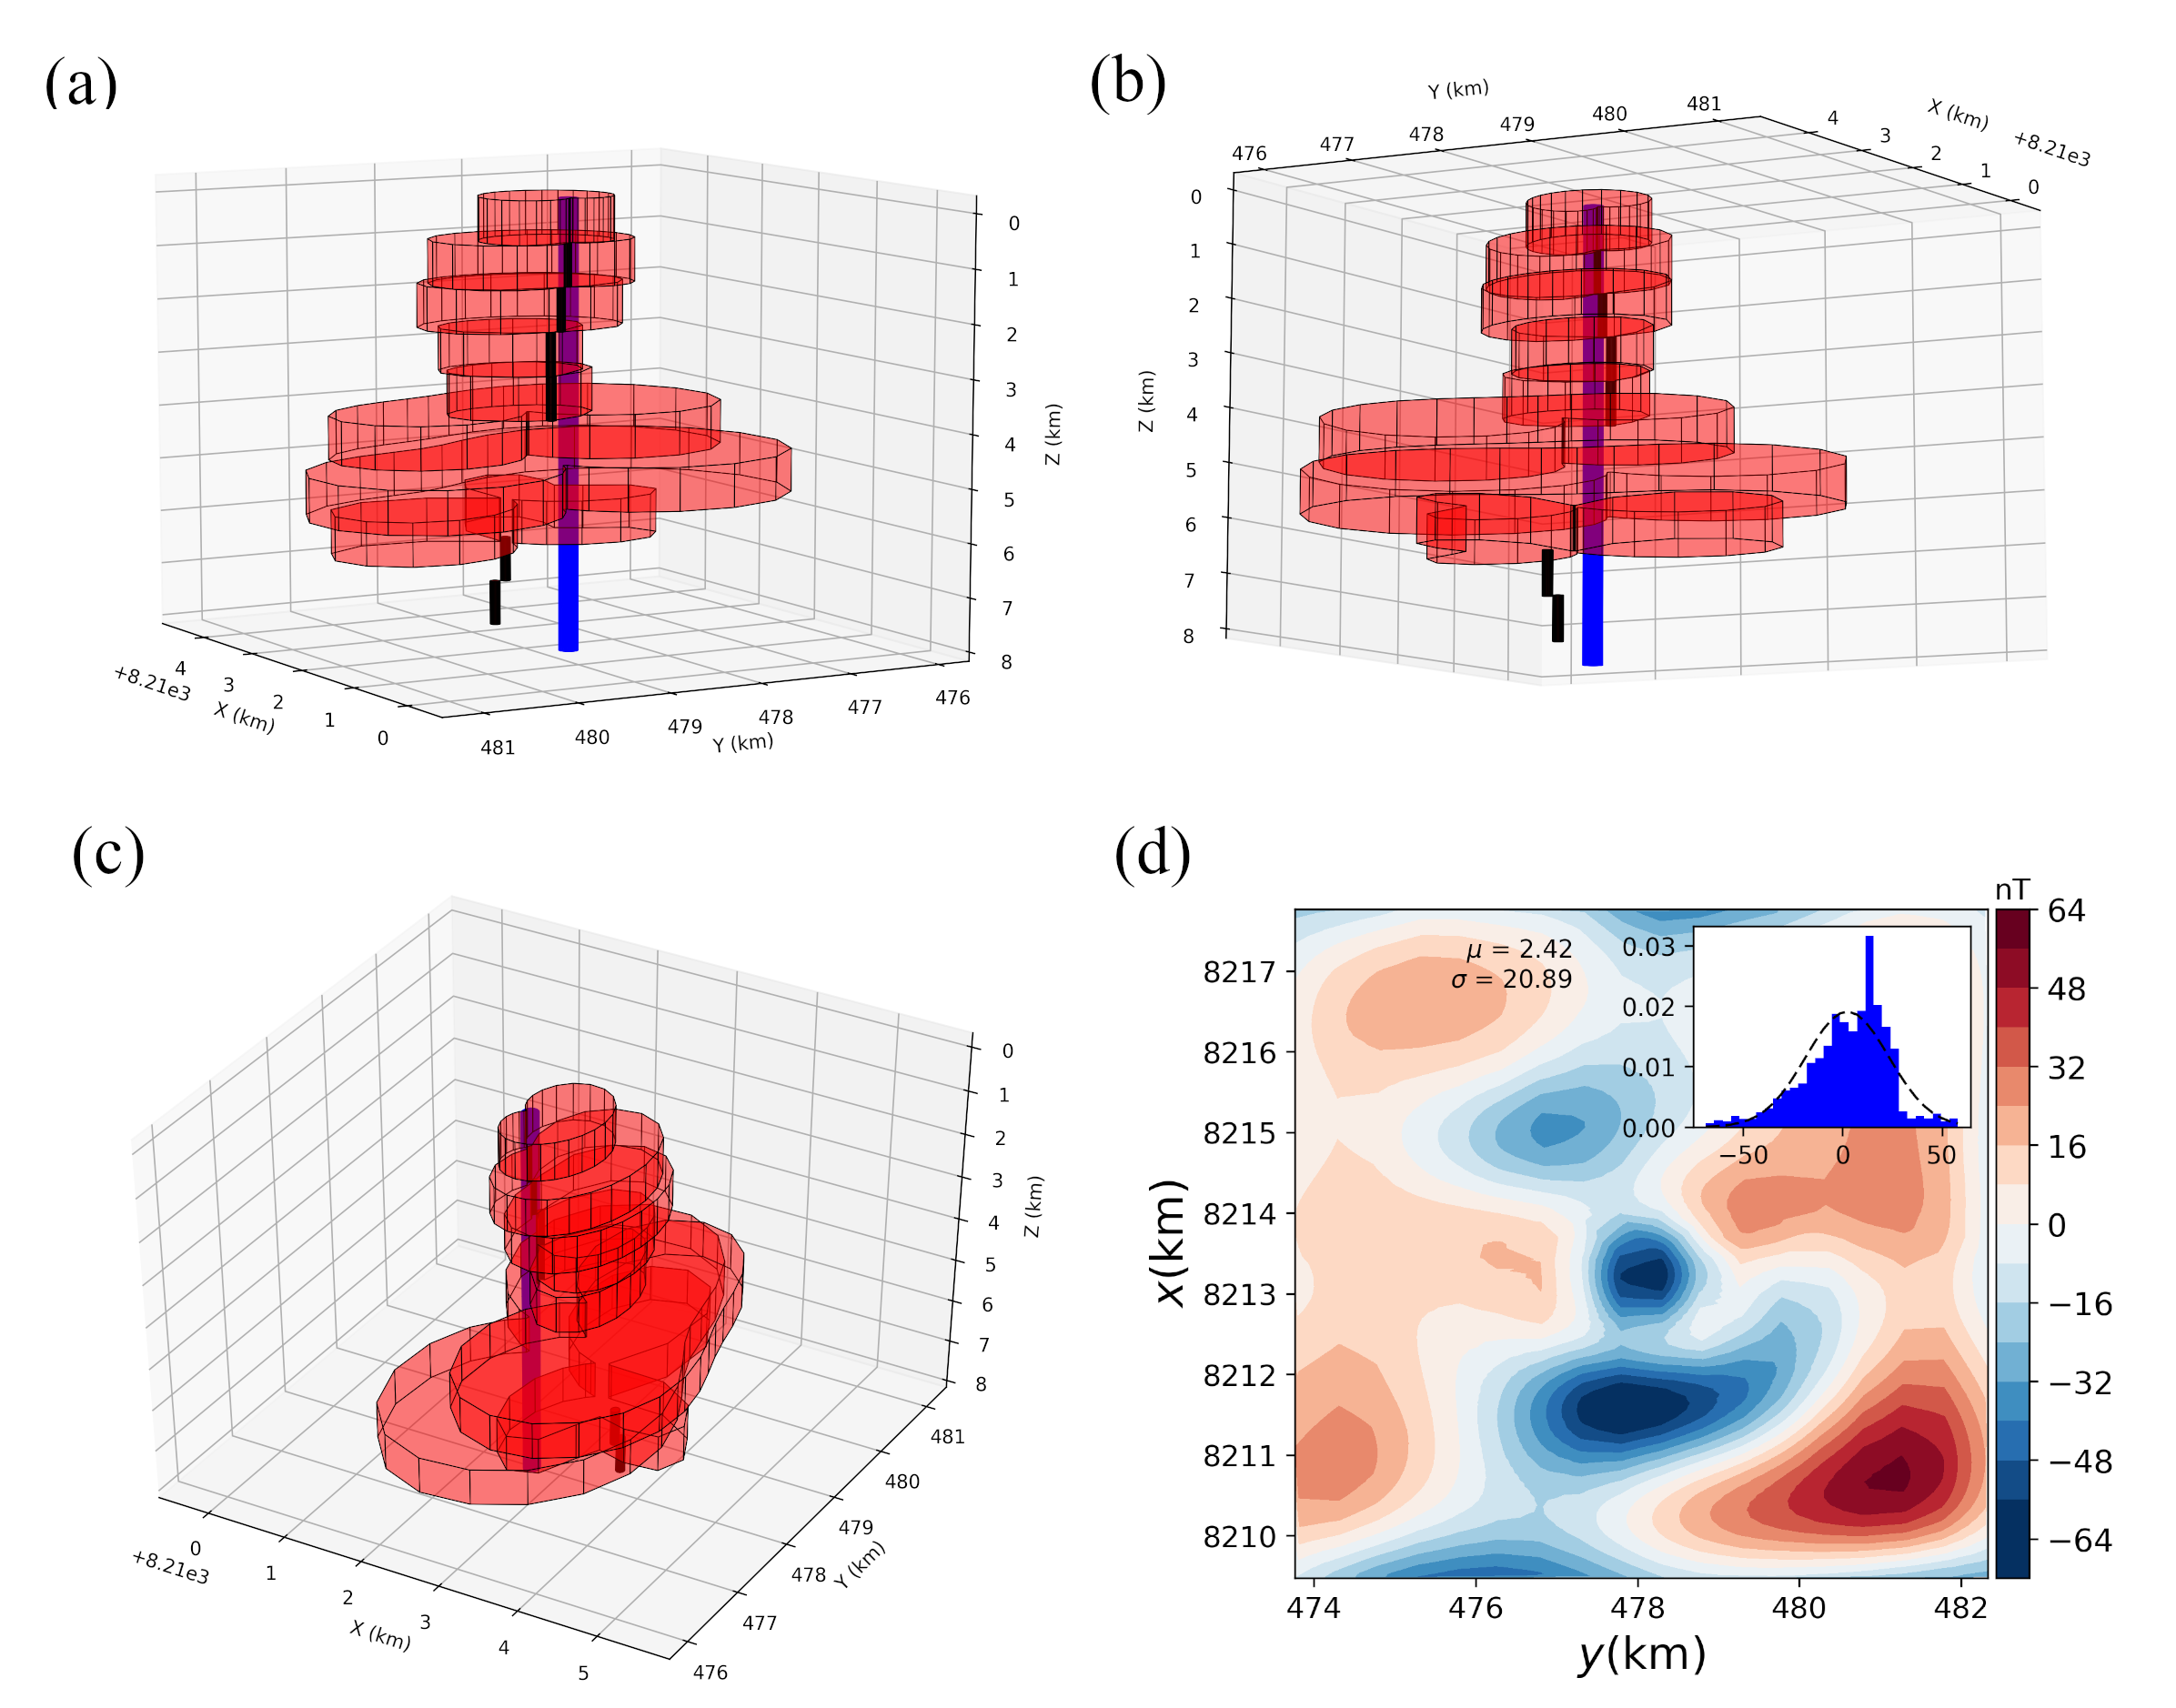
\includegraphics[scale=.75]{figures/real_data_estimates.png}
    \caption{Perspective views of the initial guess (blue cylinder) and the estimated source (red prisms) in (a), (b) and (c). (d) Residuals defined as the difference between the noisy and the predicted (not shown) total-field anomalies and the histogram of the residuals (inset in d) with mean $\mu=2.42$ nT and standard deviation $\sigma=20.89$ nT. The dashed line on the inset is the Gaussian curve for the residuals.
}
    \label{fig:real_result}
\end{figure}

\section{Conclusions}

\begin{acknowledgments}
\end{acknowledgments}

\bibliographystyle{gji}
\bibliography{ref}

\appendix

\label{lastpage}


\end{document}